\documentclass[]{elsarticle} %review=doublespace preprint=single 5p=2 column
%%% Begin My package additions %%%%%%%%%%%%%%%%%%%
\usepackage[hyphens]{url}

  \journal{SoftwareX} % Sets Journal name


\usepackage{lineno} % add

\usepackage{graphicx}
%%%%%%%%%%%%%%%% end my additions to header

\usepackage[T1]{fontenc}
\usepackage{lmodern}
\usepackage{amssymb,amsmath}
\usepackage{ifxetex,ifluatex}
\usepackage{fixltx2e} % provides \textsubscript
% use upquote if available, for straight quotes in verbatim environments
\IfFileExists{upquote.sty}{\usepackage{upquote}}{}
\ifnum 0\ifxetex 1\fi\ifluatex 1\fi=0 % if pdftex
  \usepackage[utf8]{inputenc}
\else % if luatex or xelatex
  \usepackage{fontspec}
  \ifxetex
    \usepackage{xltxtra,xunicode}
  \fi
  \defaultfontfeatures{Mapping=tex-text,Scale=MatchLowercase}
  \newcommand{\euro}{€}
\fi
% use microtype if available
\IfFileExists{microtype.sty}{\usepackage{microtype}}{}
\bibliographystyle{elsarticle-harv}
\ifxetex
  \usepackage[setpagesize=false, % page size defined by xetex
              unicode=false, % unicode breaks when used with xetex
              xetex]{hyperref}
\else
  \usepackage[unicode=true]{hyperref}
\fi
\hypersetup{breaklinks=true,
            bookmarks=true,
            pdfauthor={},
            pdftitle={Microxanox - an R package for simulating an MICRobial ecosystem that can occupy OXic or ANOXic states.},
            colorlinks=true,
            urlcolor=blue,
            linkcolor=blue,
            pdfborder={0 0 0}}
\urlstyle{same}  % don't use monospace font for urls

\setcounter{secnumdepth}{0}
% Pandoc toggle for numbering sections (defaults to be off)
\setcounter{secnumdepth}{0}

% Pandoc syntax highlighting
\usepackage{color}
\usepackage{fancyvrb}
\newcommand{\VerbBar}{|}
\newcommand{\VERB}{\Verb[commandchars=\\\{\}]}
\DefineVerbatimEnvironment{Highlighting}{Verbatim}{commandchars=\\\{\}}
% Add ',fontsize=\small' for more characters per line
\usepackage{framed}
\definecolor{shadecolor}{RGB}{248,248,248}
\newenvironment{Shaded}{\begin{snugshade}}{\end{snugshade}}
\newcommand{\AlertTok}[1]{\textcolor[rgb]{0.94,0.16,0.16}{#1}}
\newcommand{\AnnotationTok}[1]{\textcolor[rgb]{0.56,0.35,0.01}{\textbf{\textit{#1}}}}
\newcommand{\AttributeTok}[1]{\textcolor[rgb]{0.77,0.63,0.00}{#1}}
\newcommand{\BaseNTok}[1]{\textcolor[rgb]{0.00,0.00,0.81}{#1}}
\newcommand{\BuiltInTok}[1]{#1}
\newcommand{\CharTok}[1]{\textcolor[rgb]{0.31,0.60,0.02}{#1}}
\newcommand{\CommentTok}[1]{\textcolor[rgb]{0.56,0.35,0.01}{\textit{#1}}}
\newcommand{\CommentVarTok}[1]{\textcolor[rgb]{0.56,0.35,0.01}{\textbf{\textit{#1}}}}
\newcommand{\ConstantTok}[1]{\textcolor[rgb]{0.00,0.00,0.00}{#1}}
\newcommand{\ControlFlowTok}[1]{\textcolor[rgb]{0.13,0.29,0.53}{\textbf{#1}}}
\newcommand{\DataTypeTok}[1]{\textcolor[rgb]{0.13,0.29,0.53}{#1}}
\newcommand{\DecValTok}[1]{\textcolor[rgb]{0.00,0.00,0.81}{#1}}
\newcommand{\DocumentationTok}[1]{\textcolor[rgb]{0.56,0.35,0.01}{\textbf{\textit{#1}}}}
\newcommand{\ErrorTok}[1]{\textcolor[rgb]{0.64,0.00,0.00}{\textbf{#1}}}
\newcommand{\ExtensionTok}[1]{#1}
\newcommand{\FloatTok}[1]{\textcolor[rgb]{0.00,0.00,0.81}{#1}}
\newcommand{\FunctionTok}[1]{\textcolor[rgb]{0.00,0.00,0.00}{#1}}
\newcommand{\ImportTok}[1]{#1}
\newcommand{\InformationTok}[1]{\textcolor[rgb]{0.56,0.35,0.01}{\textbf{\textit{#1}}}}
\newcommand{\KeywordTok}[1]{\textcolor[rgb]{0.13,0.29,0.53}{\textbf{#1}}}
\newcommand{\NormalTok}[1]{#1}
\newcommand{\OperatorTok}[1]{\textcolor[rgb]{0.81,0.36,0.00}{\textbf{#1}}}
\newcommand{\OtherTok}[1]{\textcolor[rgb]{0.56,0.35,0.01}{#1}}
\newcommand{\PreprocessorTok}[1]{\textcolor[rgb]{0.56,0.35,0.01}{\textit{#1}}}
\newcommand{\RegionMarkerTok}[1]{#1}
\newcommand{\SpecialCharTok}[1]{\textcolor[rgb]{0.00,0.00,0.00}{#1}}
\newcommand{\SpecialStringTok}[1]{\textcolor[rgb]{0.31,0.60,0.02}{#1}}
\newcommand{\StringTok}[1]{\textcolor[rgb]{0.31,0.60,0.02}{#1}}
\newcommand{\VariableTok}[1]{\textcolor[rgb]{0.00,0.00,0.00}{#1}}
\newcommand{\VerbatimStringTok}[1]{\textcolor[rgb]{0.31,0.60,0.02}{#1}}
\newcommand{\WarningTok}[1]{\textcolor[rgb]{0.56,0.35,0.01}{\textbf{\textit{#1}}}}

% tightlist command for lists without linebreak
\providecommand{\tightlist}{%
  \setlength{\itemsep}{0pt}\setlength{\parskip}{0pt}}

% From pandoc table feature
\usepackage{longtable,booktabs,array}
\usepackage{calc} % for calculating minipage widths
% Correct order of tables after \paragraph or \subparagraph
\usepackage{etoolbox}
\makeatletter
\patchcmd\longtable{\par}{\if@noskipsec\mbox{}\fi\par}{}{}
\makeatother
% Allow footnotes in longtable head/foot
\IfFileExists{footnotehyper.sty}{\usepackage{footnotehyper}}{\usepackage{footnote}}
\makesavenoteenv{longtable}

% Pandoc citation processing
\newlength{\cslhangindent}
\setlength{\cslhangindent}{1.5em}
\newlength{\csllabelwidth}
\setlength{\csllabelwidth}{3em}
\newlength{\cslentryspacingunit} % times entry-spacing
\setlength{\cslentryspacingunit}{\parskip}
% for Pandoc 2.8 to 2.10.1
\newenvironment{cslreferences}%
  {}%
  {\par}
% For Pandoc 2.11+
\newenvironment{CSLReferences}[2] % #1 hanging-ident, #2 entry spacing
 {% don't indent paragraphs
  \setlength{\parindent}{0pt}
  % turn on hanging indent if param 1 is 1
  \ifodd #1
  \let\oldpar\par
  \def\par{\hangindent=\cslhangindent\oldpar}
  \fi
  % set entry spacing
  \setlength{\parskip}{#2\cslentryspacingunit}
 }%
 {}
\usepackage{calc}
\newcommand{\CSLBlock}[1]{#1\hfill\break}
\newcommand{\CSLLeftMargin}[1]{\parbox[t]{\csllabelwidth}{#1}}
\newcommand{\CSLRightInline}[1]{\parbox[t]{\linewidth - \csllabelwidth}{#1}\break}
\newcommand{\CSLIndent}[1]{\hspace{\cslhangindent}#1}

%% \documentclass[preprint,12pt, a4paper]{elsarticle}

%% Use the option review to obtain double line spacing
%% \documentclass[authoryear,preprint,review,12pt]{elsarticle}

%% For including figures, graphicx.sty has been loaded in
%% elsarticle.cls. If you prefer to use the old commands
%% please give \usepackage{epsfig}

%% The amssymb package provides various useful mathematical symbols
\usepackage{amssymb}
%% The amsthm package provides extended theorem environments
%% \usepackage{amsthm}

%% The lineno packages adds line numbers. Start line numbering with
%% \begin{linenumbers}, end it with \end{linenumbers}. Or switch it on
%% for the whole article with \linenumbers.
\usepackage{lineno}

\usepackage{float}
\restylefloat{table}

\journal{SoftwareX}

%\usepackage{lineno}
%\linenumbers
%\usepackage{setspace}
%\doublespacing
%\usepackage{fancyhdr}
%\fancyhead{}
%\fancyfoot{}
%\fancyhead[CO,CE]{Microxanox R package}
%\pagestyle{fancy}
%



\begin{document}


\begin{frontmatter}

  \title{Microxanox - an R package for simulating an \(MICR\)obial
ecosystem that can occupy \(OX\)ic or \(ANOX\)ic states.}
    \author[University of Zürich]{Rainer M Krug\corref{Corresponding
Author}}
   \ead{Rainer.Krug@uzh.ch \& Rainer@krugs.de} 
    \author[University of Zürich]{Owen L. Petchey}
   \ead{Owen.Petchey@ieu.uzh.ch} 
      \address[University of Zürich]{Department of Evolutionary Biology
and Environmental Studies, Winterthurerstrasse 190, 8057 Zurich}
      \cortext[1]{Corresponding Author}
    \cortext[2]{Equal contribution}
  
  \begin{abstract}
  Ca. 100 words.
  \end{abstract}
   \begin{keyword} metadata quality; data curation; archival; long term
storage; R package;\end{keyword}
 \end{frontmatter}

\hypertarget{required-metadata}{%
\section{Required Metadata}\label{required-metadata}}

\hypertarget{current-code-version}{%
\subsection{Current code version}\label{current-code-version}}

Ancillary data table required for subversion of the codebase.

\begin{longtable}[]{@{}
  >{\raggedright\arraybackslash}p{(\columnwidth - 4\tabcolsep) * \real{0.3333}}
  >{\raggedright\arraybackslash}p{(\columnwidth - 4\tabcolsep) * \real{0.3333}}
  >{\raggedright\arraybackslash}p{(\columnwidth - 4\tabcolsep) * \real{0.3333}}@{}}
\toprule
\begin{minipage}[b]{\linewidth}\raggedright
\textbf{Nr.}
\end{minipage} & \begin{minipage}[b]{\linewidth}\raggedright
\textbf{Code metadata description}
\end{minipage} & \begin{minipage}[b]{\linewidth}\raggedright
\textbf{Please fill in this column}
\end{minipage} \\
\midrule
\endhead
C1 & Current code version & For example v42 \\
C2 & Permanent link to code/repository used for this code version &
\url{https://github.com/UZH-PEG/microxanox} \\
C3 & Code Ocean compute capsule & \\
C4 & Legal Code License & CC BY 4.0 \\
C5 & Code versioning system used & git \\
C6 & Software code languages, tools, and services used & R \\
C7 & Compilation requirements, operating environments & R (\textgreater=
4.1.0), ADD PACKAGES \\
C8 & If available Link to developer documentation/manual & \\
C9 & Support email for questions & Rainer.Krug@uzh.ch;
Rainer@krugs.de \\
\bottomrule
\end{longtable}

\hypertarget{motivation-and-significance}{%
\section{Motivation and
significance}\label{motivation-and-significance}}

Introduce the scientific background and the motivation for developing
the software. Explain why the software is important, and describe the
exact (scientific) problem(s) it solves. Indicate in what way the
software has contributed (or how it will con- tribute in the future) to
the process of scientific discovery; if available, this is to be
supported by citing a research paper using the software. Provide a
description of the experimental setting (how does the user use the
software?). Introduce related work in literature (cite or list
algorithms used, other software etc.).

\hypertarget{software-description}{%
\section{Software description}\label{software-description}}

Describe the software in as much as is necessary to establish a
vocabulary needed to explain its impact.

\hypertarget{software-architecture}{%
\subsection{Software Architecture}\label{software-architecture}}

Give a short overview of the overall software architecture; provide a
pic- torial component overview or similar (if possible). If necessary
provide im- plementation details.

\hypertarget{software-functionalities}{%
\subsection{Software Functionalities}\label{software-functionalities}}

Present the major functionalities of the software.

\hypertarget{illustrative-examples}{%
\section{Illustrative Examples}\label{illustrative-examples}}

Provide at least one illustrative example to demonstrate the major
functions. Optional: you may include one explanatory video that will
appear next to your article, in the right hand side panel.

\hypertarget{impact}{%
\section{Impact}\label{impact}}

This is the main section of the article and the reviewers weight the
description here appropriately Indicate in what way new research
questions can be pursued as a result of the software (if any). Indicate
in what way, and to what extent, the pursuit of existing research
questions is improved (if so). Indicate in what way the software has
changed the daily practice of its users (if so). Indicate how widespread
the use of the software is within and outside the intended user group.
Indicate in what way the software is used in commercial settings and/or
how it led to the creation of spin-off companies (if so).

\hypertarget{conclusions}{%
\section{Conclusions}\label{conclusions}}

Set out the conclusion of this original software publication.

\hypertarget{conflict-of-interest}{%
\section{Conflict of Interest}\label{conflict-of-interest}}

We wish to confirm that there are no known conflicts of interest
associated with this publication and there has been no significant
financial support for this work that could have influenced its outcome.

\hypertarget{acknowledgements}{%
\section{Acknowledgements}\label{acknowledgements}}

Optionally thank people and institutes you need to acknowledge.

\hypertarget{introduction}{%
\section{Introduction}\label{introduction}}

{\{\textgreater\textgreater Biological justification and background -
one paragraph - DONE\textless\textless\} }

Many ecosystems are exposed to gradual changes of environmental
variables, to which the responses are not always as gradual as the
change of the environmental variable. One example where the gradual
change of a single environmental causing an abrupt change of the system
is the switch from an aerobic to anaerobic system. This system hass been
investigated by Bush et al. (\protect\hyperlink{ref-Bush2017}{2017}). We
wanted to take this investigation one step further, and look at the role
of an increased biodiversity plays in these dynamics
(\protect\hyperlink{ref-REF_NEEDED}{REF NEEDED, 2222}). For this
purpose, we developed this package.

The microxanox package is a package for simulating a three functional
group system (\emph{CB}: cyanobacteria, \emph{PB}: phototrophic sulfur
bacteria, and \emph{SB}: sulfate-reducing bacteria) with four chemical
substrates (\emph{P}: phosphorus, \emph{O}: oxygen, \emph{SR}: reduced
sulfur, \emph{SO}: oxidized sulfur). It includes feddback between
biogeochemical processes and is based on
(\protect\hyperlink{ref-Bush2017}{Bush et al., 2017}) (See
(\protect\hyperlink{ref-Bush2017}{Bush et al., 2017}) for a detailed
discussion of the model).

The aims of the \texttt{microxanox} package are twofold. Firstly, the
package aims at reproducing the results shown by
(\protect\hyperlink{ref-Bush2017}{Bush et al., 2017}), which is
acomplished in the \href{LINK\%20NEEDED}{vignette Partial reproduction
of Bush et al}. Secondly, to take these results one step further, it
includes new functionality to adress our research question as presented
in (\protect\hyperlink{ref-REF_NEEDED}{REF NEEDED, 2222}).

For this, we extended the model and added functionality for:

\begin{itemize}
\tightlist
\item
  Multiple strains (effectively unlimited) per functional group.
\item
  Adding temporally varying oxygen diffusivity.
\item
  Adding random noise in substrate concentrations.
\item
  Including immigration.
\item
  Setting minimum population abundances.
\end{itemize}

In addition to the model itself, the package includes some functions to
analyse the results as well as visualise the results to provide a
starting point for customised visualisations based on own requirements.

\hypertarget{general-usability-and-flexibility-of-the-model}{%
\subsection{General usability and flexibility of the
model}\label{general-usability-and-flexibility-of-the-model}}

The package is not intended to provide a modelling framework which can
be adjusted easily to all needs, but primarily a tool to implement the
model used by (\protect\hyperlink{ref-Bush2017}{Bush et al., 2017}) and
to extend it to our needs (\protect\hyperlink{ref-REF_NEEDED}{REF
NEEDED, 2222}). Consequently, any more substantial changes and
adaptaitions, are likely to need a change in the source code.

Nevertheless, the model is structured in a way which builds on a modular
structuere, so that e.g.~the event definition can easily be changed. or
other aspects can be adjusted. All values in the parameter object can be
changed as needed and the general structure of the code should make it
not to difficult to adapt the model to other similar systems.

\hypertarget{the-model}{%
\section{The Model}\label{the-model}}

The model is an implementation of the model described by
(\protect\hyperlink{ref-Bush2017}{Bush et al., 2017}). It is an ordinary
differential equation (ODE) based numerical non-stochastic model which
was implemented in form of an R package.

We use the notation from the \href{LINK\%20NEEDED}{Table S1} of the
Supplementary information of (\protect\hyperlink{ref-Bush2017}{Bush et
al., 2017})), and not the notation in the main manuscript of
(\protect\hyperlink{ref-Bush2017}{Bush et al., 2017}). In the main
manuscript the notation is simplified to \texttt{y\_S\_PB}
(\(y_{S,PB}\)) (which is \texttt{y\_SR\_PB} (\(y_{SR,PB}\)) in Table S1)
and \texttt{y\_S\_SB} (\(y_{S,SB}\)) (which is y\_SO\_SB (\(y_{SO,SB}\))
in Table S1). We also use \texttt{Pr\_cB} (\(Pr_B\)) instead of
\texttt{P\_CB} (\(P_{CB}\)).

All parameter and variables follow these base dimensions:

\begin{itemize}
\tightlist
\item
  Time: \texttt{hours}
\item
  Volume: \texttt{litres}
\item
  Substrate quantity: \texttt{micromoles}
\item
  Organism quantity: \texttt{cells}
\end{itemize}

{\{\textgreater\textgreater{} Add a more detailed description of the
model and the additions \textless\textless\}
\{\textgreater\textgreater TODO\textless\textless\}}

The ODEs are solved using the ``General Solver for Ordinary Differential
Equations'' of the \texttt{deSolve} package
(\protect\hyperlink{ref-Soetaert2010}{Soetaert et al., 2010}).

\hypertarget{availability-and-accessability-of-the-package}{%
\section{Availability and Accessability of the
package}\label{availability-and-accessability-of-the-package}}

The package is available in a
\href{https://github.com/UZH-PEG/microxanox/}{github repo/}. The newest
version is also available under the \href{https://DOI}{DOI} or via
RUniverse (\protect\hyperlink{ref-REF_NEEDED}{REF NEEDED, 2222}). This
manuscript describes version 1.0 which is available under
\href{https://DOI}{DOI} or installable within R by using
\texttt{remotes::install\_github("UZH-PEG",\ ref\ =\ "v1.0")}.

The package will be updated based on further research activities. It
will be tested continuously for the last recent, current and devel
version of R. {\{\textgreater\textgreater If we want that, we have to
include some, even rudimentary, GITHUB tests.\textless\textless\}
\{\textgreater\textgreater RMK: Agreed - let's discuss this when we talk
about the package paper.\textless\textless\} }

Issues, questions and suggestions should be communicated through the
issue tracker at \url{https://github.com/UZH-PEG/microxanox/issues}

\hypertarget{package-description}{%
\section{Package description}\label{package-description}}

\hypertarget{documentation}{%
\subsection{Documentation}\label{documentation}}

The package contains the full documentetion of the functions, which
includes

\begin{enumerate}
\def\labelenumi{\arabic{enumi}.}
\tightlist
\item
  Standard R help for each function (\texttt{?COMMAND} in R)
\item
  Two vignettes acompanying the package:
\end{enumerate}

\begin{itemize}
\tightlist
\item
  A \textbf{User Guide}, also available on the R-Universe
  \href{@LINK_NEEDED}{Vignette 1}. This gives an introduction of the
  package and its functions and provides a walk-through of the process
  of running, visualizing and extra and \href{@LINK_NEEDED}{Vignette 2}
\end{itemize}

\begin{enumerate}
\def\labelenumi{\arabic{enumi}.}
\setcounter{enumi}{2}
\tightlist
\item
  This paper as a third vignette, also available under RUniverse
  \href{@LINK_NEEDED}{Vignette 3}
\end{enumerate}

\hypertarget{reproducibility}{%
\subsection{Reproducibility}\label{reproducibility}}

The framework used when writing this package aims at reproducibility of
the results. It builds on the folowing main considerations:

\begin{enumerate}
\def\labelenumi{\arabic{enumi}.}
\tightlist
\item
  all parameter needed to run a simulation or find a stable state are
  contained in a single parameter object. This object is created by
  using the functions \texttt{new\_...\_parameter()},
  \texttt{new\_initial\_state()} and \texttt{new\_strain\_parameter()}.
  Which one of the \texttt{new\_...\_parameter()} functions has to be
  used when, will be discussed in the section @ref(runsim) and in the
  \href{LINK_NEEDED}{User Guide}.
\item
  The function call \texttt{run\_...(parameter)} will run the simulation
  using the parameter as defined in the object \texttt{parameter}.
\item
  The return value of the \texttt{run\_...(parameter)} function is
  identical to the parameter object plus an additionl slot named
  \texttt{results} which contains the results of the run
\item
  As this return value contains all parameter, it is possible to re-run
  the simulatuion by simply running \texttt{run\_...(result)}.
\end{enumerate}

The point that the results object contains all parameter needed to run
the simulation, promotes reproducibility and makes incremental changes
of individual parameters and re-running the simulations much easier.

A typical simulation would look as followed:

\begin{Shaded}
\begin{Highlighting}[]
\DocumentationTok{\#\# Create the parameter}
\NormalTok{parameter }\OtherTok{\textless{}{-}} \FunctionTok{new\_runsim\_parameter}\NormalTok{()}
\CommentTok{\# manually setting certain parameter}

\DocumentationTok{\#\# Run the simulation and save the result}
\NormalTok{result }\OtherTok{\textless{}{-}} \FunctionTok{run\_simulatrion}\NormalTok{(parameter)}
\FunctionTok{saveRDS}\NormalTok{(result, }\StringTok{"sim1.rds"}\NormalTok{)}

\DocumentationTok{\#\# Do other stuff, e.g. plotting}

\DocumentationTok{\#\# Load results, change some parameter, and rerun the simulation and save the result}
\NormalTok{parameter }\OtherTok{\textless{}{-}} \FunctionTok{loadRDS}\NormalTok{(}\StringTok{"sim1.rds"}\NormalTok{)}
\CommentTok{\# change some parameter}
\NormalTok{result }\OtherTok{\textless{}{-}} \FunctionTok{run\_simulatrion}\NormalTok{(parameter)}
\FunctionTok{saveRDS}\NormalTok{(result, }\StringTok{"sim2,rds"}\NormalTok{)}
\end{Highlighting}
\end{Shaded}

\hypertarget{runsim}{%
\subsection{Using the package}\label{runsim}}

We will now discuss the general structure and functiuonality of the
package without going into to much detail. A more detailed discussion
can be found in the \href{LINK_NEEDED}{User Guide}.

The ODEs for the rates of change are specified in the function
\texttt{bushplus\_dynamic\_model()}. This augmented version of the model
published in (\protect\hyperlink{ref-Bush2017}{Bush et al., 2017}) can
handle multiple strains within each of the three functional groups,
temporal variation in oxygen diffusivity, and events.

In the following sections we describe the general usage of the package:
running one simulation, finding steady states across an environmental
gradient, calculating measures of stability, and visualisation.

\hypertarget{running-one-simulation}{%
\subsubsection{Running one simulation}\label{running-one-simulation}}

The individual simulation (\texttt{run\_simulation()} function) is the
working horse in this package. In this function, the ODEs are solved.
The function needs only one argument - an object as created by the
function \texttt{new\_runsim\_parameter()}. One parameter of this object
is the \texttt{strain\_parameter} which can be created by the function
\texttt{new\_strain\_parameter()}. For a detailed description of the
parameter and how they are created please see the User Guide and which
acomnpanies the package or is available at \href{@LINK_NEEDED}{User
Guide}

After the parameter object has been defined, it can be used in the
\texttt{run\_simulation()} function. The function returns an object
which is identical to the parameter, except of an additional slot
containing the results. This design produces a fully reproducible object
as it can be used instead of a parameter object to be fed back into the
\texttt{run\_simulation()} function to run the simulation again from the
parameter used to generate the results from.

The function \texttt{plot\_dynamics()} plots a single simulation run, as
returned from the \texttt{run\_simulation()} function. This functio is
only provided as a convenience function to provide a way to easily see
the results of a simulation run. An example plot resulting from this
function is shown in @ref(fig:plot-dynamics).

\begin{figure}

{\centering 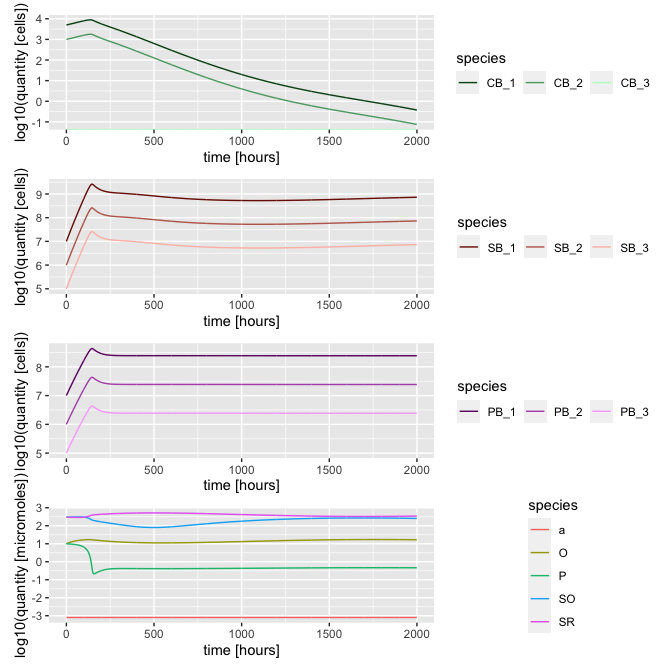
\includegraphics[width=500px]{figures/ug_three_strains_dynamics} 

}

\caption{Plot of results of a simulation run using the function $plot_dynamics()$. Details can be found in the "User Guide" section "Three strains per functional group".}\label{fig:plot-dynamics}
\end{figure}

\hypertarget{finding-a-steady-state-of-the-model}{%
\subsubsection{Finding a Steady State of the
model}\label{finding-a-steady-state-of-the-model}}

There are two methods for finding steady states. The first runs a
separate simulation for each combination of starting conditions and
oxygen diffusivity (let us term this the \emph{Replication method}). The
second runs only two simulations, with step-wise and slowly temporally
increasing or decreasing oxygen diffusivities and recorded of state just
before change to a new oxygen diffusivity (let us term this the
\emph{Temporal method}).

\hypertarget{replication-method}{%
\paragraph{Replication Method}\label{replication-method}}

The replication method is implementad in the function
\texttt{run\_replication\_ssfind()} which takes a parameter object as
returned by the function \texttt{new\_replication\_ssfind\_parameter()}
and the number of cores for multithreading the simulation.

\hypertarget{temporal-method}{%
\paragraph{Temporal Method}\label{temporal-method}}

The temporal method involves two simulations for a particular system
configuration (parameter set). In one simulation the oxygen diffusivity
is \emph{increased} in a step-wise fashion. In the other it is
\emph{decreased} in a step-wise fashion. That is, oxygen diffusivity is
held at a constant level for long enough for steady state to be reach,
that state is recorded, and then a slightly higher (or lower) oxygen
diffusivity value is set. Hence, at that time point, the system is
effectively started with initial conditions that are the state of the
system in the previous time step.

This is implemented in the function \texttt{run\_temporal\_ssfind()},
which takes a parameter object as created by the function
\texttt{new\_temporal\_ssfind\_parameter()} and a number indicating the
.

For a more detailed walk-through of these two approaches and explanation
please see the \href{@LINK_NEEDED}{User Guide}.

\hypertarget{extracting-stability-measures}{%
\subsection{Extracting Stability
Measures}\label{extracting-stability-measures}}

From the raw results returned by these \texttt{run\_...()} functions,
the stability measures can be extracted by using the function
\texttt{get\_stability\_measures()}. These measures include
non-linearity and hysteresis measures, of the response of the simulated
system to environmental change.

\hypertarget{use-cases}{%
\section{Use cases}\label{use-cases}}

The first two use cases are described in detail in the User Guide and
the Partial Reproduction Vignettes. The third is taken from the REF
NEEDED (\protect\hyperlink{ref-REF_NEEDED}{2222}) for which this R
package was designed. All of these use cases can be expanded to larger
numbers of strains per functional group and variable values van be
changed.

\hypertarget{regime-shifts-during-temporal-environmental-change}{%
\subsection{Regime shifts during temporal environmental
change}\label{regime-shifts-during-temporal-environmental-change}}

In the \href{LINK_NEEDED}{User Guide} we used a one strain system
(section ``1 strain per functional group'') and three strain system
(section ``3 strains per functional group'') to determine as an example
the stable states during temporal environmental changes (the oxygen
diffusivity). From these simulatiuons, we extracted measures of
nonlinearity and hysteresis. See Fig @ref(fig:plot-dynamics) as an
example plot of the simulations.

\begin{figure}

{\centering 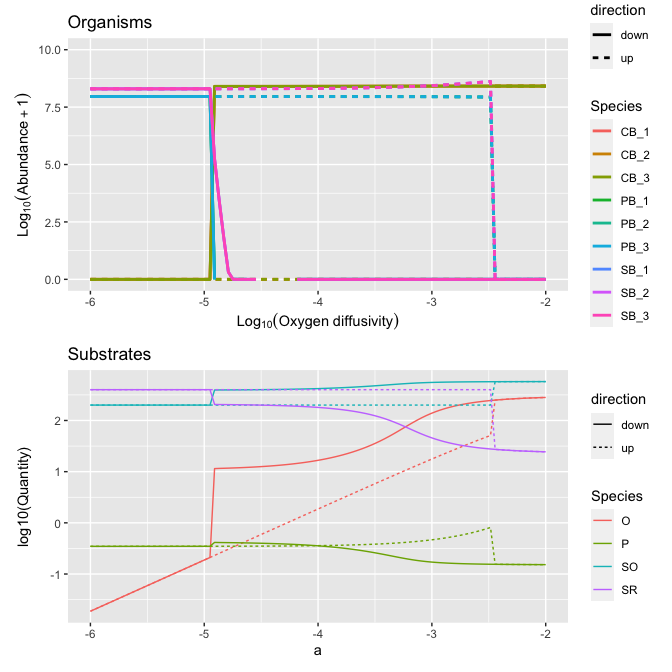
\includegraphics[width=500px]{figures/ug_three_strains_stable_state} 

}

\caption{Plot of the stable states of the simulation runs under different oxygen diffusivity. The top graph are the Organisms (ech initially with three strains) while the lower graph is the substrate availability under the same oxygen diffusivities. Details can be found in the "User Guide" section "Three strains per functional group".}\label{fig:uc1_stable_state}
\end{figure}

\hypertarget{the-extent-of-hysteresis-depends-on-community-composition}{%
\subsection{The extent of hysteresis depends on community
composition}\label{the-extent-of-hysteresis-depends-on-community-composition}}

One of the reasons to develop this package was to reproduce the results
presented in Bush et al. (\protect\hyperlink{ref-Bush2017}{2017}), this
was achieved as demonstrated in the \href{LINK_NEEDED}{Partial
Reproduction supplement}. All aspects in the paper could be reproduced
and are shown in the vignette.

\begin{figure}

{\centering 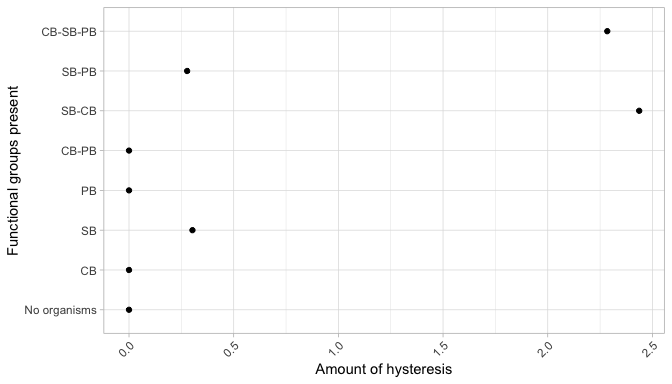
\includegraphics[width=500px]{figures/user_guide_hysteresis} 

}

\caption{Hysteresis of all assessed combinations of variability.}\label{fig:user_guide_hysteresis}
\end{figure}

\hypertarget{effects-of-functional-diversity-on-regime-shifts}{%
\subsection{Effects of functional diversity on regime
shifts}\label{effects-of-functional-diversity-on-regime-shifts}}

As discussed in the paper (\protect\hyperlink{ref-REF_NEEDED}{REF
NEEDED, 2222}), the role biodiversity plays in abrupt regime shifts
based on gradual changing environmental parameter is not well
understood. This model (as part of the package) has been used to
investigate these dynamics and the results are available in REF NEEDED
(\protect\hyperlink{ref-REF_NEEDED}{2222}).

{\{\textgreater\textgreater More details from the
paper.\textless\textless\}\\
\{\textgreater\textgreater Romana will provide two or three
sentences\textless\textless\}}

\hypertarget{conclusions-1}{%
\section{Conclusions}\label{conclusions-1}}

\{\textgreater\textgreater Dependant on journal\textless\textless\}

\hypertarget{references}{%
\section*{References}\label{references}}
\addcontentsline{toc}{section}{References}

\hypertarget{refs}{}
\begin{CSLReferences}{1}{0}
\leavevmode\vadjust pre{\hypertarget{ref-Bush2017}{}}%
Bush, T., Diao, M., Allen, R.J., Sinnige, R., Muyzer, G., Huisman, J.,
2017. Oxic-anoxic regime shifts mediated by feedbacks between
biogeochemical processes and microbial community dynamics. Nature
Communications 8, 789.
doi:\href{https://doi.org/10.1038/s41467-017-00912-x}{10.1038/s41467-017-00912-x}

\leavevmode\vadjust pre{\hypertarget{ref-REF_NEEDED}{}}%
REF NEEDED, A., 2222. {REFERNECE NEEDED}. Journal of missing references.

\leavevmode\vadjust pre{\hypertarget{ref-Soetaert2010}{}}%
Soetaert, K., Petzoldt, T., Setzer, R.W., 2010. Solving differential
equations in {R}: {Package deSolve}. Journal of Statistical Software 33,
1--25.
doi:\href{https://doi.org/10.18637/jss.v033.i09}{10.18637/jss.v033.i09}

\end{CSLReferences}


\end{document}
